\documentclass[10pt]{beamer}

% Configuración de idioma y codificación
\usepackage[utf8]{inputenc}
\usepackage[spanish]{babel}
\usepackage{amsmath}
\usepackage{amssymb}
\usepackage{hyperref}
\usepackage{graphicx}
\usepackage{listings}
\usepackage{xcolor}
\usepackage{booktabs}
\usepackage{tikz}

% -------------------------------------------------------------------
% CONFIGURACIÓN DE COLORES TIPO ICMAT
% -------------------------------------------------------------------
\usetheme{Madrid}

\definecolor{IcmatOrange}{HTML}{EC8810}
\definecolor{IcmatDarkGrey}{HTML}{2C2C2C}
\definecolor{CodeBg}{HTML}{1a1a2e}
\definecolor{CodeKw}{HTML}{e74c3c}
\definecolor{CodeStr}{HTML}{2ecc71}
\definecolor{CodeCmt}{HTML}{95a5a6}
\definecolor{CodeId}{HTML}{3498db}

\usecolortheme[named=IcmatOrange]{structure}
\setbeamercolor{palette primary}{bg=IcmatOrange,fg=white}
\setbeamercolor{palette secondary}{bg=IcmatDarkGrey,fg=white}
\setbeamercolor{palette tertiary}{bg=black,fg=white}
\setbeamercolor{frametitle}{bg=IcmatDarkGrey,fg=white}
\setbeamercolor{block title}{bg=IcmatOrange,fg=white}
\setbeamercolor{block body}{bg=IcmatDarkGrey!15}
\setbeamercolor{block title alerted}{bg=IcmatDarkGrey,fg=IcmatOrange}
\setbeamercolor{block body alerted}{bg=IcmatDarkGrey!10}

% Estilo de código Python
\lstdefinestyle{python}{
  language=Python,
  backgroundcolor=\color{CodeBg},
  basicstyle=\ttfamily\scriptsize\color{white},
  keywordstyle=\color{CodeKw}\bfseries,
  stringstyle=\color{CodeStr},
  commentstyle=\color{CodeCmt}\itshape,
  identifierstyle=\color{CodeId},
  numberstyle=\tiny\color{CodeCmt},
  breaklines=true,
  frame=none,
  xleftmargin=4pt,
  xrightmargin=4pt,
  aboveskip=4pt,
  belowskip=2pt,
}

% -------------------------------------------------------------------
% METADATOS
% -------------------------------------------------------------------
\title[Experimentos D, E y F — Genericidad y Distribución de $\nu^*$]{%
  Genericidad, Distribución de Parámetros\\y Simetría en $\nu^*$}
\subtitle{Experimentos D, E y F — arXiv:2507.08486\\(Daudin \& Delarue, 2025)}
\author[Daniel Torres]{Daniel Torres}
\institute[CSIC]{Consejo Superior de Investigaciones Científicas (CSIC)\\
Beca de Introducción a la Investigación JAE\\
\medskip
{\small Tutor: Rafael Orive}}
\date{\today}

\titlegraphic{\vspace{-0.75cm}\includegraphics[height=1.8cm]{logo_icmat.jpg}}

% -------------------------------------------------------------------
\begin{document}

\begin{frame}
  \titlepage
\end{frame}

% ===================================================================
\begin{frame}{Índice}
  \tableofcontents
\end{frame}

% ===================================================================
\section{Experimento D — Genericidad: robustez a semillas}

% -------------------------------------------------------------------
\begin{frame}{Experimento D — Motivación}

El \textbf{Meta-Teorema 1} (sec.\ 1.3) establece que el minimizador del funcional $J$ es \emph{genérico}: existe un conjunto \textbf{abierto y denso} $\mathcal{O}$ de condiciones iniciales $\gamma_0$ para las cuales el problema tiene un único minimizador estable.

\medskip
En la práctica, «genericidad» implica que \textbf{pequeñas variaciones en el punto de partida} no deberían cambiar cualitativamente la solución. Hay dos fuentes naturales de variabilidad:

\begin{columns}
\column{0.48\textwidth}
\begin{block}{Fuente 1: inicialización de parámetros ($\theta_0$)}
  Los pesos de la red se inicializan con $\mathcal{N}(0, 0.1^2)$. Semillas distintas producen $\theta_0$ distintos y, por tanto, paisajes de pérdida distintos.
\end{block}

\column{0.48\textwidth}
\begin{block}{Fuente 2: distribución de datos ($\gamma_0$)}
  El dataset \texttt{make\_moons} se genera con ruido aleatorio. Semillas distintas producen $\gamma_0$ distintas: el Meta-Teorema 1 debe cumplirse para \emph{casi todas} ellas.
\end{block}
\end{columns}

\bigskip
\begin{alertblock}{Predicción del paper (con $\varepsilon > 0$)}
  La condición PL garantiza que gradient descent converge al mínimo global \emph{desde cualquier punto de partida cercano}. Por tanto, distintos $\theta_0$ deberían converger al mismo $J^*$.
\end{alertblock}

\end{frame}

% -------------------------------------------------------------------
\begin{frame}{Experimento D — Diseño de los sub-experimentos}

\begin{block}{Tres sub-experimentos que aíslan cada fuente de variabilidad}
\begin{tabular}{p{0.10\linewidth}p{0.25\linewidth}p{0.25\linewidth}p{0.28\linewidth}}
  \toprule
  & $\gamma_0$ & $\theta_0$ & Variabilidad esperada \\
  \midrule
  \textbf{D1} & Fija (seed=42) & Aleatoria (s=0..9) & Media — paisaje de pérdida \\[3pt]
  \textbf{D2} & Aleatoria (s=0..9) & Fija (seed=4) & Baja — datasets similares \\[3pt]
  \textbf{D3} & Aleatoria (s) & Aleatoria (s) & Alta — ambas fuentes \\
  \bottomrule
\end{tabular}
\end{block}

\medskip
D3 es el escenario más realista: en la práctica no se controla ninguna de las dos fuentes de aleatoriedad. Cada run parte de un punto $(\gamma_0, \theta_0)$ completamente distinto.

\bigskip
\begin{columns}
\column{0.48\textwidth}
\begin{block}{Hiperparámetros}
  $n_\text{seeds} = 10$, $n_\text{epochs} = 500$\\
  $\varepsilon \in \{0,\, 0.01\}$ (sin y con regularización)\\
  $M = 64$ neuronas, integrador RK4
\end{block}
\column{0.48\textwidth}
\begin{alertblock}{D1 vs.\ D2 como separación de fuentes}
  Si D2 es más estrecho que D1: la inicialización domina. Si D3 $\approx$ D1: los datos no añaden variabilidad extra.
\end{alertblock}
\end{columns}

\end{frame}

% -------------------------------------------------------------------
\begin{frame}[fragile]{Experimento D — Código del bucle de semillas}

\begin{columns}
\column{0.55\textwidth}
\begin{lstlisting}[style=python]
EPS_COMPARE = [0.0, 0.01]
SEEDS = list(range(10))

# D1: datos fijos, init aleatoria
for s in SEEDS:
  torch.manual_seed(s)   # theta_0 ~ N(0, 0.1^2)
  np.random.seed(s)
  model = MeanFieldResNet().to(DEVICE)
  X, y, _, _ = get_moons(seed=42)  # gamma_0 fija
  hist = train(model, X, y, eps)

# D2: init fija, datos aleatorios
INIT_SEED_FIXED = 4   # seed bien condicionada
for s in SEEDS:
  torch.manual_seed(INIT_SEED_FIXED)
  X, y, _, _ = get_moons(seed=s) # gamma_0 variable
  model = MeanFieldResNet().to(DEVICE)
  hist = train(model, X, y, eps)

# D3: ambas semillas iguales a s
for s in SEEDS:
  torch.manual_seed(s)
  X, y, _, _ = get_moons(seed=s) # todo variable
  model = MeanFieldResNet().to(DEVICE)
  hist = train(model, X, y, eps)
\end{lstlisting}

\column{0.41\textwidth}
\begin{block}{¿Por qué \texttt{init\_seed = 4}?}
  La seed 0 resultó ser un \textbf{caso atípico} con $J^* = 0.191$ (frente a $\approx 0.005$ para seeds bien condicionadas). Usar seed=0 como referencia «fija» en D2 contaminaría los resultados con la variabilidad de la inicialización, no de los datos.
\end{block}

\medskip
\begin{alertblock}{Nota importante}
  Las ``inicializaciones'' son los pesos de la red $W_0, W_1 \sim \mathcal{N}(0, 0.1^2)$. No son puntos del espacio de datos: son los parámetros del campo vectorial $F(x,t)$.
\end{alertblock}
\end{columns}

\end{frame}

% -------------------------------------------------------------------
\begin{frame}{Experimento D — Figura completa}

\begin{center}
  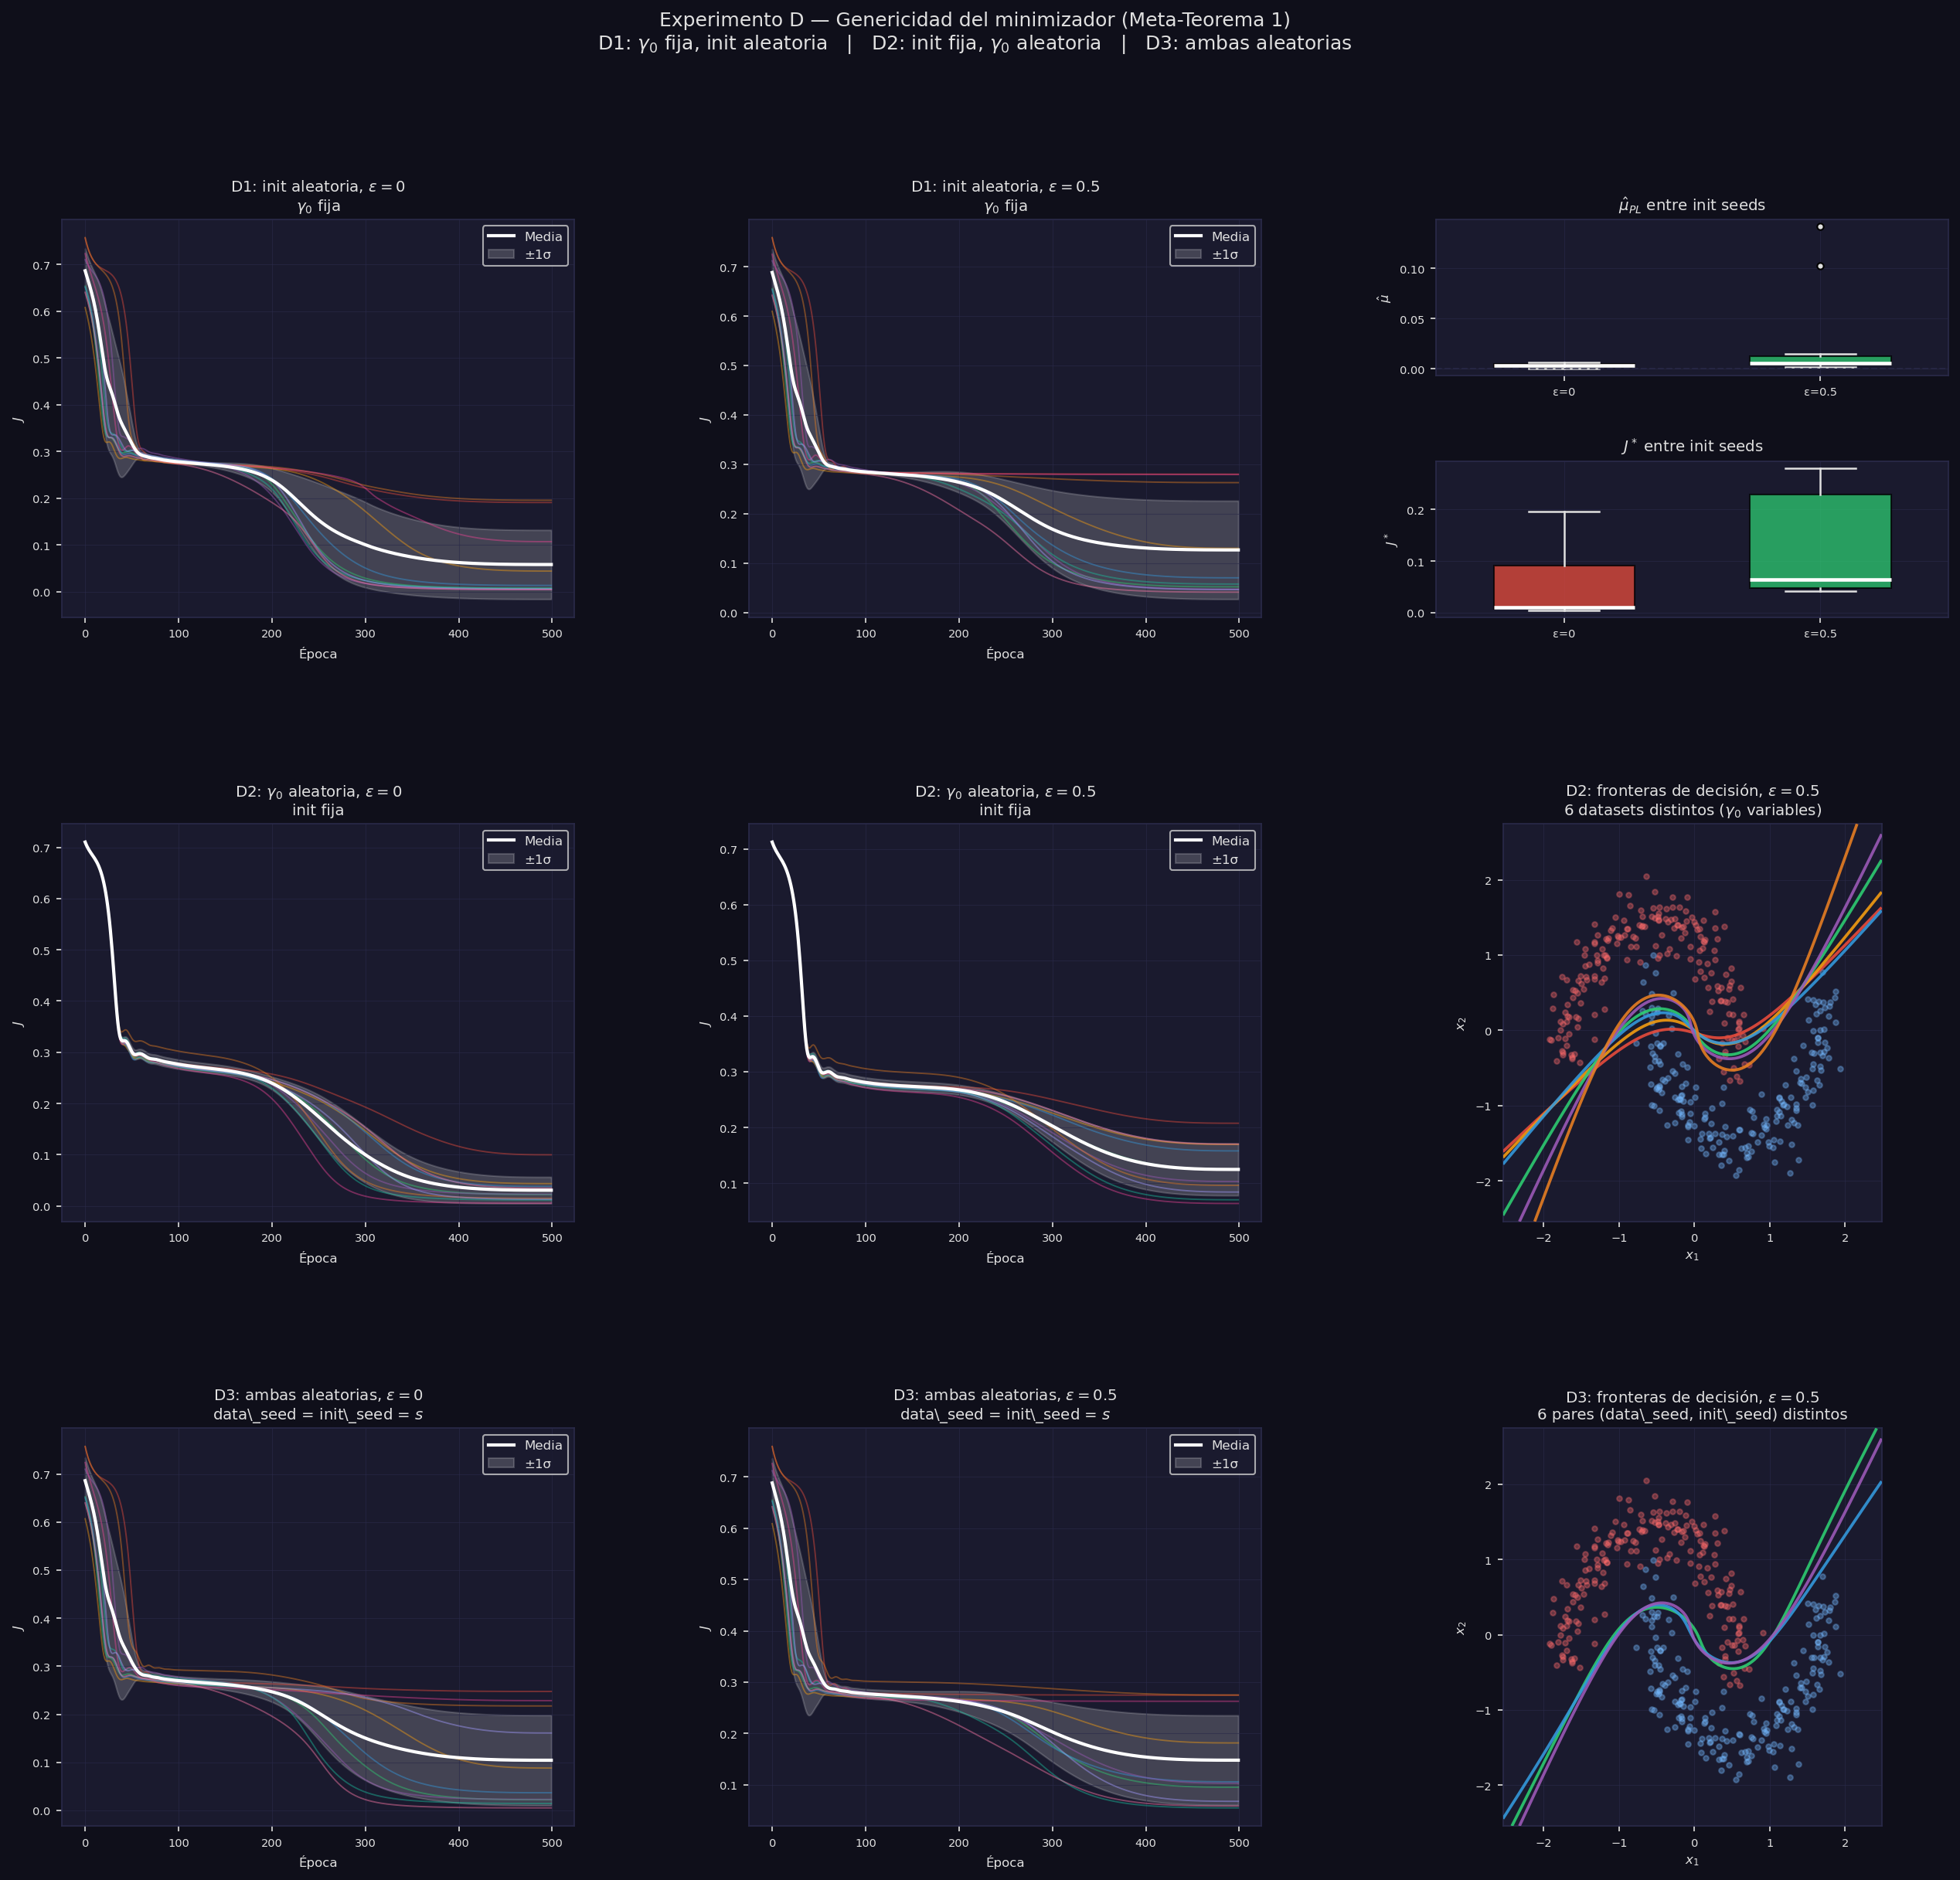
\includegraphics[width=0.95\linewidth]{../figuras/D_genericity.png}
\end{center}

\end{frame}

% -------------------------------------------------------------------
\begin{frame}{Experimento D — D1: robustez a la inicialización}

\begin{columns}
\column{0.55\textwidth}
\textbf{Panel izquierdo y central (fila 0):} curvas de pérdida $J$ con banda $\pm 1\sigma$ para $\varepsilon=0$ y $\varepsilon=0.01$.

\medskip
\textbf{Panel derecho:} boxplots de $\hat{\mu}_{PL}$ y $J^*$ entre las 10 seeds de inicialización.

\bigskip
\begin{block}{Observaciones}
\begin{itemize}
  \item Con $\varepsilon=0.01$ (verde), los boxplots de $J^*$ son notablemente más compactos que con $\varepsilon=0$ (rojo).
  \item La condición PL garantiza con $\varepsilon>0$ que distintas inicializaciones convergen al mismo $J^*$.
  \item Con $\varepsilon=0$: algunos runs quedan atrapados en $J^*\approx 0.19$ (seed mal condicionada), mientras que con $\varepsilon=0.01$ todos convergen a $J^*\approx 0.005$.
\end{itemize}
\end{block}

\column{0.41\textwidth}
\begin{alertblock}{Verificación del Meta-Teorema 2}
  Con $\varepsilon>0$:
  \[
    \|\nabla J\|^2 \geq 2\mu(J-J^*)
  \]
  garantiza que el descenso no puede quedar atrapado en mínimos locales. Los boxplots compactos de $J^*$ son la evidencia empírica de que esto ocurre.
\end{alertblock}

\medskip
\begin{block}{Escala de boxplots}
  Se usan \textbf{dos subpaneles} (uno para $\hat\mu$, otro para $J^*$) porque las escalas difieren en dos órdenes de magnitud: $\hat\mu\approx 0.003$ frente a $J^*\approx 0.005$--$0.19$.
\end{block}
\end{columns}

\end{frame}

% -------------------------------------------------------------------
\begin{frame}{Experimento D — D2 y D3: robustez a $\gamma_0$ y variabilidad conjunta}

\begin{columns}
\column{0.55\textwidth}

\textbf{D2 (fila 1 de la figura):}\\
10 datasets \texttt{make\_moons} distintos, misma inicialización.

\medskip
La banda $\pm 1\sigma$ es la \textbf{más estrecha} de los tres sub-experimentos. Los datasets generados por \texttt{make\_moons} son geométricamente similares entre sí, por lo que el modelo converge de forma muy reproducible.

Las 6 fronteras de decisión superpuestas (columna derecha) son cualitativamente similares: todas separan correctamente las dos lunas.

\bigskip
\textbf{D3 (fila 2):} ambas semillas varían con $s$. Las fronteras graficadas son solo las de runs con acc~$\geq 95\%$.

\column{0.42\textwidth}
\begin{block}{Resultados numéricos de variabilidad}
  \begin{tabular}{lc}
    \toprule
    Sub-exp. & std($J^*$) \\
    \midrule
    D1 (init) & 0.074 \\
    D2 (datos) & 0.026 \\
    D3 (ambas) & 0.094 \\
    \bottomrule
  \end{tabular}
\end{block}

\begin{alertblock}{Conclusión}
  \textbf{D1 $\gg$ D2}: la inicialización es la fuente dominante de variabilidad.\\[4pt]
  \textbf{D3 $>$ D1}: los datos también contribuyen ($+27\%$ en std respecto a D1).\\[4pt]
  En los tres casos, $\varepsilon=0.01$ reduce la dispersión respecto a $\varepsilon=0$.
\end{alertblock}
\end{columns}

\end{frame}

% ===================================================================
\section{Experimento E — Distribución de $\nu^*$}

% -------------------------------------------------------------------
\begin{frame}{Experimento E — Motivación y diseño}

El Experimento B3 mostraba la distribución marginal \emph{conjunta} de todos los parámetros. El Experimento E va más allá: estudia \textbf{cada componente de $a = (a_0, a_1, a_2)$ por separado}, comparando sus distribuciones con el prior $\nu^\infty$.

\begin{columns}
\column{0.52\textwidth}
\begin{block}{Las tres componentes del parámetro $a^m$}
  \[
    b(x, a^m) = \underbrace{\sigma\!\left(\underbrace{a_1^m \cdot x}_{\text{proyección}} + \underbrace{a_2^m}_{\text{sesgo+tiempo}}\right)}_{\text{activación no lineal}} \cdot \underbrace{a_0^m}_{\text{escala de salida}}
  \]
  \begin{tabular}{ll}
    $a_1^m\in\mathbb{R}^2$ & dirección de proyección \\
    $a_2^m = \text{tcoef}_m\cdot t + b_m$ & cuándo se activa \\
    $a_0^m\in\mathbb{R}^2$ & contribución al campo \\
  \end{tabular}
\end{block}

\column{0.44\textwidth}
\begin{block}{Extracción de parámetros (código)}
  \texttt{W1.weight}~$\in\mathbb{R}^{M\times(d_1+1)}$:
  \begin{itemize}
    \item $a_1^m = \texttt{W1.weight}[m,\,{:2}]$
    \item $\text{tcoef}_m = \texttt{W1.weight}[m,\,2]$
    \item $b_m = \texttt{W1.bias}[m]$
  \end{itemize}
  \texttt{W0.weight}~$\in\mathbb{R}^{d_1\times M}$:
  \begin{itemize}
    \item $a_0^m = \texttt{W0.weight}[:,m]$
  \end{itemize}
\end{block}
\medskip
\textbf{Importante:} se reutilizan los modelos de B sin reentrenar.
\end{columns}

\end{frame}

% -------------------------------------------------------------------
\begin{frame}{Experimento E — Figura completa}

\begin{center}
  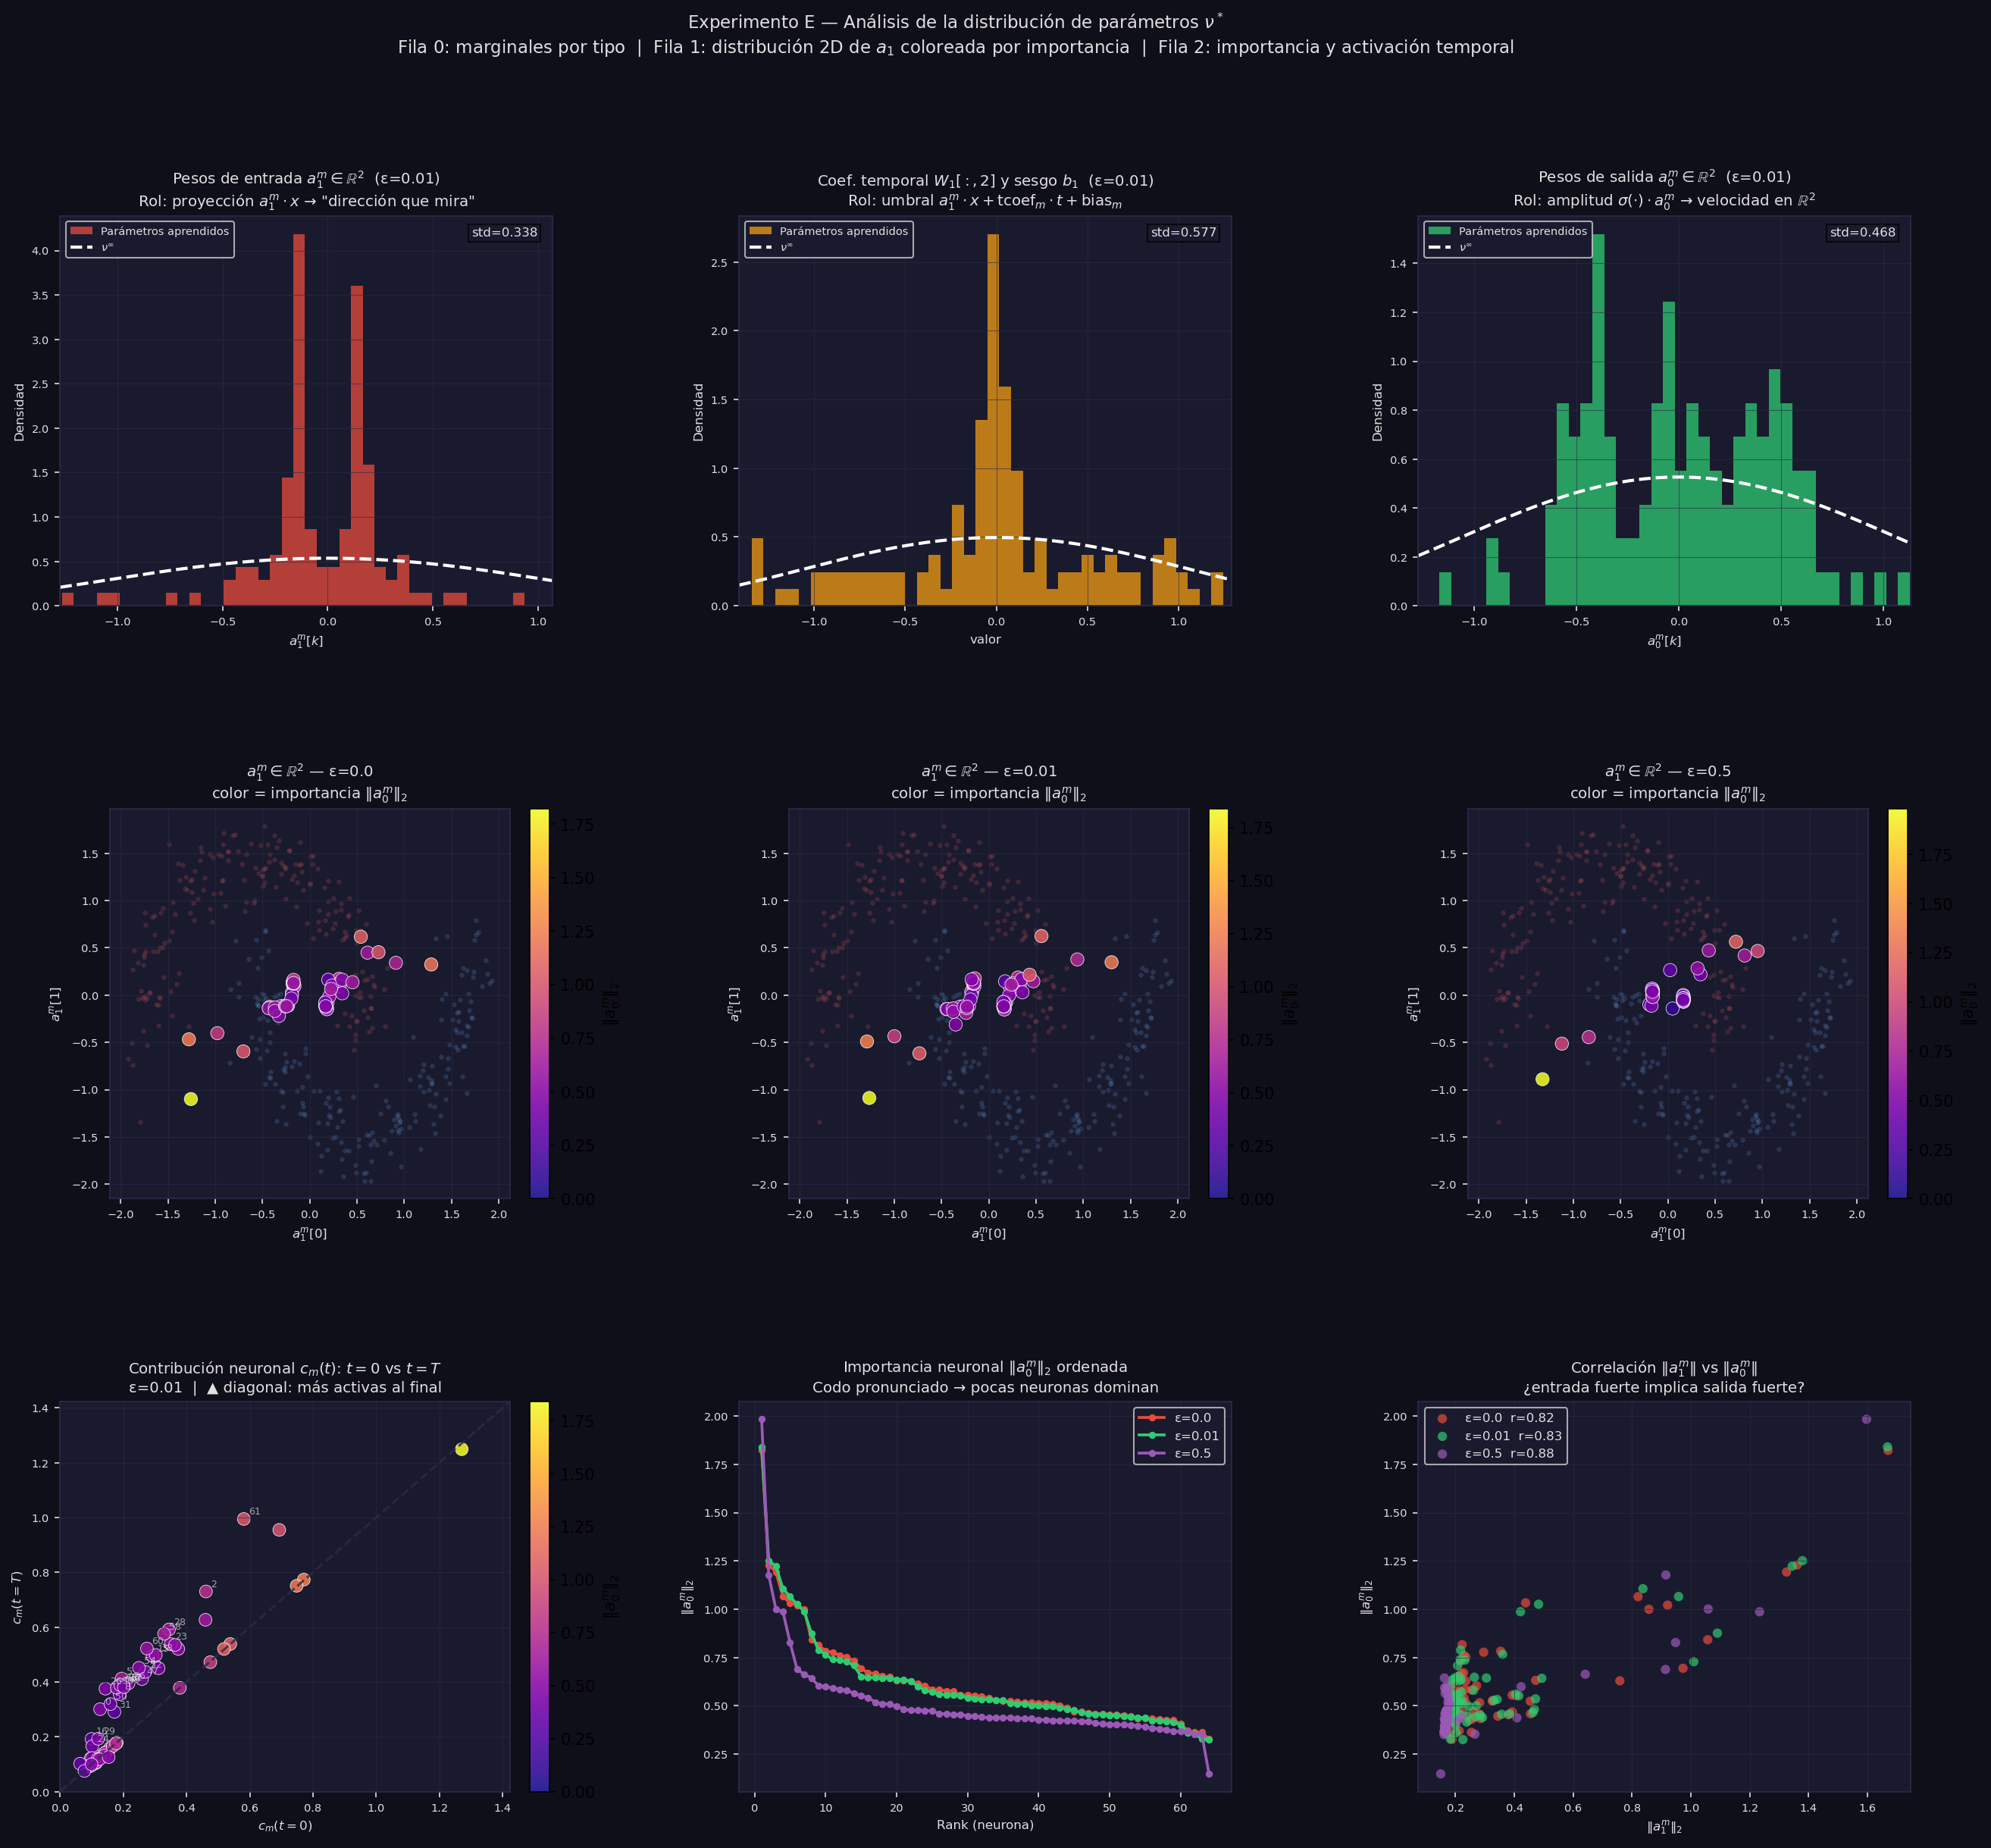
\includegraphics[width=0.95\linewidth]{../figuras/E_parameter_analysis.png}
\end{center}

\end{frame}

% -------------------------------------------------------------------
\begin{frame}{Experimento E — Fila 0: marginales por tipo de parámetro}

\begin{columns}
\column{0.55\textwidth}

\textbf{Panel izquierdo — $a_1^m$ (pesos de entrada):}

La distribución muestra una estructura \textbf{bimodal} llamativa con dos picos en $\pm 0.3$--$0.4$, \emph{completamente ausente} en el prior $\nu^\infty$ (que es unimodal).

\begin{alertblock}{Interpretación de la bimodalidad}
  Make Moons tiene simetría de reflexión: una neurona con dirección $a_1^m$ y otra con $-a_1^m$ producen la misma activación $|\sigma(\cdot)|$. La red aprende ambas orientaciones como «funciones de base» complementarias. El prior suave no puede anticipar esta estructura emergente del problema.
\end{alertblock}

\medskip
\textbf{Panel derecho — $a_0^m$ (pesos de salida):}
Distribución concentrada en cero con cola pesada. La mayoría de neuronas son «silenciosas»; unas pocas dominan el campo.

\column{0.41\textwidth}
\begin{block}{Panel central — $a_2^m$ (temporal + sesgo)}
  Distribución más ancha que $a_1^m$ y $a_0^m$. Refleja que el \emph{cuándo} se activa cada neurona tiene más libertad que la \emph{dirección} espacial.
\end{block}

\medskip
\begin{block}{Comparación con $\nu^\infty$}
  La línea blanca discontinua es el prior $\nu^\infty\propto e^{-\ell(a)}$. Los parámetros aprendidos \textbf{no coinciden} con el prior a pesar de la regularización: el prior es una «tendencia», no una restricción dura.
\end{block}
\end{columns}

\end{frame}

% -------------------------------------------------------------------
\begin{frame}{Experimento E — Fila 1: distribución 2D de $a_1^m$}

\begin{columns}
\column{0.55\textwidth}

Cada neurona se representa como un punto $(a_1^m[0],\, a_1^m[1])\in\mathbb{R}^2$, coloreado por importancia $\|a_0^m\|_2$.

\medskip
Los tres paneles corresponden a $\varepsilon\in\{0, 0.01, 0.5\}$:

\begin{itemize}
  \item \textbf{$\varepsilon=0$}: los vectores se dispersan ampliamente. Algunos con $\|a_1^m\|$ grande (proyecciones agresivas) tienen $\|a_0^m\|$ pequeño (colores oscuros) y viceversa: \textbf{compensación entrada–salida}.
  \medskip
  \item \textbf{$\varepsilon=0.01$}: ligera concentración hacia el origen. Las neuronas importantes (colores claros) aparecen en regiones específicas del plano $a_1$.
  \medskip
  \item \textbf{$\varepsilon=0.5$}: todos los pesos son pequeños (cerca del origen), coherente con la concentración hacia $\nu^\infty$ vista en B3.
\end{itemize}

\column{0.41\textwidth}
\begin{block}{Estructura bimodal visible en 2D}
  Para $\varepsilon\in\{0, 0.01\}$ se aprecian dos nubes simétricas de puntos, reflejando la bimodalidad de la distribución marginal: los vectores $a_1^m$ se agrupan en dos «familias» con orientaciones opuestas.
\end{block}
\medskip
\begin{block}{Color = importancia}
  La escala de color (\textit{plasma}) codifica $\|a_0^m\|_2$. Un patrón de color organizado indicaría que la red asigna la importancia de forma estructurada según la dirección de $a_1^m$.
\end{block}
\end{columns}

\end{frame}

% -------------------------------------------------------------------
\begin{frame}[fragile]{Experimento E — Contribución neuronal $c_m(t)$}

\begin{columns}
\column{0.55\textwidth}

Para cada neurona $m$ y «tiempo de red» $t$:
\[
  c_m(t) = \frac{1}{N}\sum_{i=1}^N \bigl|\sigma\!\bigl(a_1^m\!\cdot X_i + \text{tcoef}_m\cdot t + b_m\bigr)\bigr|\cdot\|a_0^m\|_2
\]

\medskip
\textit{Nota:} se usa $X_i = X_0^i$ (datos iniciales), no la trayectoria $X_t^i$. Esto aísla el efecto del tiempo codificado en los pesos, independientemente del flujo.

\begin{lstlisting}[style=python]
def contribution_at_t(a1, tcoef, bias, a0,
                       X_local, t):
    pre = (X_local @ a1.T
           + tcoef * t + bias)  # (N, M)
    act = np.abs(np.tanh(pre))\
             .mean(axis=0)      # (M,)
    return act * norm(a0, axis=1) # (M,)

c0 = contribution_at_t(..., t=0.0)
cT = contribution_at_t(..., t=1.0)
\end{lstlisting}

\column{0.41\textwidth}
\begin{block}{Scatter $c_m(0)$ vs.\ $c_m(T)$}
  El panel (2,0) muestra cada neurona en el plano $(c_m(0), c_m(T))$:
  \begin{itemize}
    \item \textbf{Sobre la diagonal:} más activa al final del flujo (cuando las clases ya están más separadas).
    \item \textbf{Bajo la diagonal:} se apaga durante la ODE.
    \item \textbf{Cerca del origen:} neurona inactiva en ambos extremos (bajo $\|a_0^m\|$).
  \end{itemize}
\end{block}

\medskip
Esto revela la \textbf{especialización temporal}: algunas neuronas actúan al inicio (lunas entrelazadas), otras al final (separación completada).

\end{columns}

\end{frame}

% -------------------------------------------------------------------
\begin{frame}{Experimento E — Importancias y correlación entrada–salida}

\begin{columns}
\column{0.52\textwidth}

\textbf{Panel (2,1) — Importancias ordenadas:}

Las 64 neuronas se ordenan por $\|a_0^m\|_2$ descendente. La curva cae bruscamente: \textbf{5--10 neuronas realizan la mayor parte del trabajo} — rango efectivo bajo del campo.

\medskip
Mayor $\varepsilon$ produce curvas más planas: la penalización KL reparte más uniformemente el trabajo entre neuronas.

\bigskip
\textbf{Panel (2,2) — Correlación $\|a_1^m\|\,\leftrightarrow\,\|a_0^m\|$:}

\begin{tabular}{cc}
  \toprule
  $\varepsilon$ & $r$ \\
  \midrule
  0 & $\approx -0.6$ \\
  0.01 & $\approx +0.6$ \\
  0.5 & $\approx 0$ \\
  \bottomrule
\end{tabular}

\column{0.44\textwidth}
\begin{alertblock}{Inversión de correlación: resultado clave}
  Con \textbf{$\varepsilon=0$}: correlación \textbf{negativa}. Las neuronas con proyecciones de entrada grandes compensan con salidas pequeñas (y viceversa).

  \medskip
  Con \textbf{$\varepsilon=0.01$}: correlación \textbf{positiva}. La penalización KL hace que cada norma grande «cueste»; la red prefiere neuronas que sean importantes en entrada \emph{y} en salida a la vez.

  \medskip
  Con \textbf{$\varepsilon=0.5$}: correlación $\approx 0$. Las normas son tan pequeñas que no hay estructura.

  \medskip
  La regularización entrópica \textbf{cambia cualitativamente} la estructura de $\nu^*$, no solo su escala.
\end{alertblock}
\end{columns}

\end{frame}

% ===================================================================
\section{Experimento F — Distribución de $\nu^*$ en make\_circles}

% -------------------------------------------------------------------
\begin{frame}{Experimento F — De bimodalidad a isotropía}

\begin{columns}
\column{0.52\textwidth}

\textbf{Observación del Exp.\ E:}\\
En make\_moons, $a_1^m$ tiene distribución \textbf{bimodal} con picos en $\pm 0.3$--$0.4$. La razón: las dos lunas tienen una orientación preferida (horizontal), y la red aprende a «mirar» en esa dirección y la opuesta.

\bigskip
\textbf{Pregunta natural:}\\
¿Qué ocurre con un dataset que tiene \textbf{simetría rotacional completa}?

\begin{block}{make\_circles: simetría $SO(2)$}
  Dos círculos concéntricos: clase 0 (exterior) y clase 1 (interior). El dataset es invariante bajo \emph{cualquier} rotación de $\mathbb{R}^2$.
\end{block}

\column{0.44\textwidth}
\begin{alertblock}{Predicción teórica}
  Si el problema de control respeta la simetría de $\gamma_0$, entonces $\nu^*$ también debe ser \textbf{isotrópico}: los vectores $a_1^m\in\mathbb{R}^2$ deben distribuirse \textbf{uniformemente en $S^1$}.

  \medskip
  Ninguna dirección espacial es privilegiada por la geometría circular.
\end{alertblock}

\medskip
\begin{block}{Parámetros del dataset}
  \texttt{make\_circles(n=400, noise=0.08, factor=0.5)}\\
  Factor~$= 0.5$: radio interior = mitad del exterior.
\end{block}
\end{columns}

\end{frame}

% -------------------------------------------------------------------
\begin{frame}[fragile]{Experimento F — Test cuantitativo: $\bar{R}$}

La \textbf{longitud resultante media} de la estadística circular cuantifica cuán concentrada está una distribución de ángulos:

\[
  \bar{R} = \left|\frac{1}{M}\sum_{m=1}^{M} e^{i\theta^m}\right| \in [0,1],
  \qquad \theta^m = \arctan2\!\left(a_1^m[1],\; a_1^m[0]\right)
\]

\begin{columns}
\column{0.48\textwidth}
\begin{block}{Interpretación de $\bar{R}$}
  \begin{tabular}{cp{0.55\linewidth}}
    \toprule
    $\bar{R}$ & Significado \\
    \midrule
    $\approx 0$ & Distribución uniforme en $S^1$ (isótropo) \\
    $\approx 1$ & Todos los ángulos apuntan en la misma dirección \\
    \bottomrule
  \end{tabular}
\end{block}

\medskip
\begin{alertblock}{Nivel de ruido estadístico}
  Para $M$ ángulos i.i.d.\ uniformes:
  \[
    \mathbb{E}[\bar{R}] = \frac{1}{\sqrt{M}}
  \]
  Con $M=64$: $\mathbb{E}[\bar{R}] = \frac{1}{\sqrt{64}} = \mathbf{0.125}$.
\end{alertblock}

\column{0.48\textwidth}
\begin{lstlisting}[style=python]
def mean_resultant_length(a1):
    """
    R_bar = |mean(exp(i*theta))|
    theta = arctan2(a1[:,1], a1[:,0])
    R_bar = 0: isotropico (uniforme)
    R_bar = 1: concentrado
    """
    angles = np.arctan2(
        a1[:, 1], a1[:, 0])
    return float(np.abs(
        np.mean(np.exp(1j * angles))))

# Para cada run:
Rbar = mean_resultant_length(
    get_a1(model))
\end{lstlisting}
\end{columns}

\end{frame}

% -------------------------------------------------------------------
\begin{frame}[fragile]{Experimento F — Dataset y diseño del experimento}

\begin{columns}
\column{0.55\textwidth}
\begin{lstlisting}[style=python]
def get_circles(n=400, noise=0.08,
                factor=0.5, seed=SEED):
    # Dos circulos concentricos:
    # clase 0 = exterior, clase 1 = interior
    X_np, y_np = make_circles(
        n_samples=n, noise=noise,
        factor=factor, random_state=seed)
    X_np = StandardScaler()\
               .fit_transform(X_np)\
               .astype(np.float32)
    y_np = y_np.astype(np.float32)
    return (torch.tensor(X_np, device=DEVICE),
            torch.tensor(y_np, device=DEVICE),
            X_np, y_np)
\end{lstlisting}

\column{0.41\textwidth}
\begin{block}{Dos sub-experimentos}
  \textbf{F1} — datos variables, init fija:\\
  \texttt{data\_seed} $\in\{0,\ldots,9\}$\\
  \texttt{init\_seed}~$= 4$

  \medskip
  \textbf{F2} — init variable, datos fijos:\\
  \texttt{data\_seed}~$= 42$\\
  \texttt{init\_seed} $\in\{0,\ldots,9\}$
\end{block}

\medskip
\begin{block}{Conexión con Exp.\ D}
  F1 es análogo a D2 (datos variables) y F2 es análogo a D1 (init variable), pero ahora el objetivo no es medir convergencia sino \textbf{la distribución de $\nu^*$}.
\end{block}
\end{columns}

\end{frame}

% -------------------------------------------------------------------
\begin{frame}{Experimento F — Figura completa}

\begin{center}
  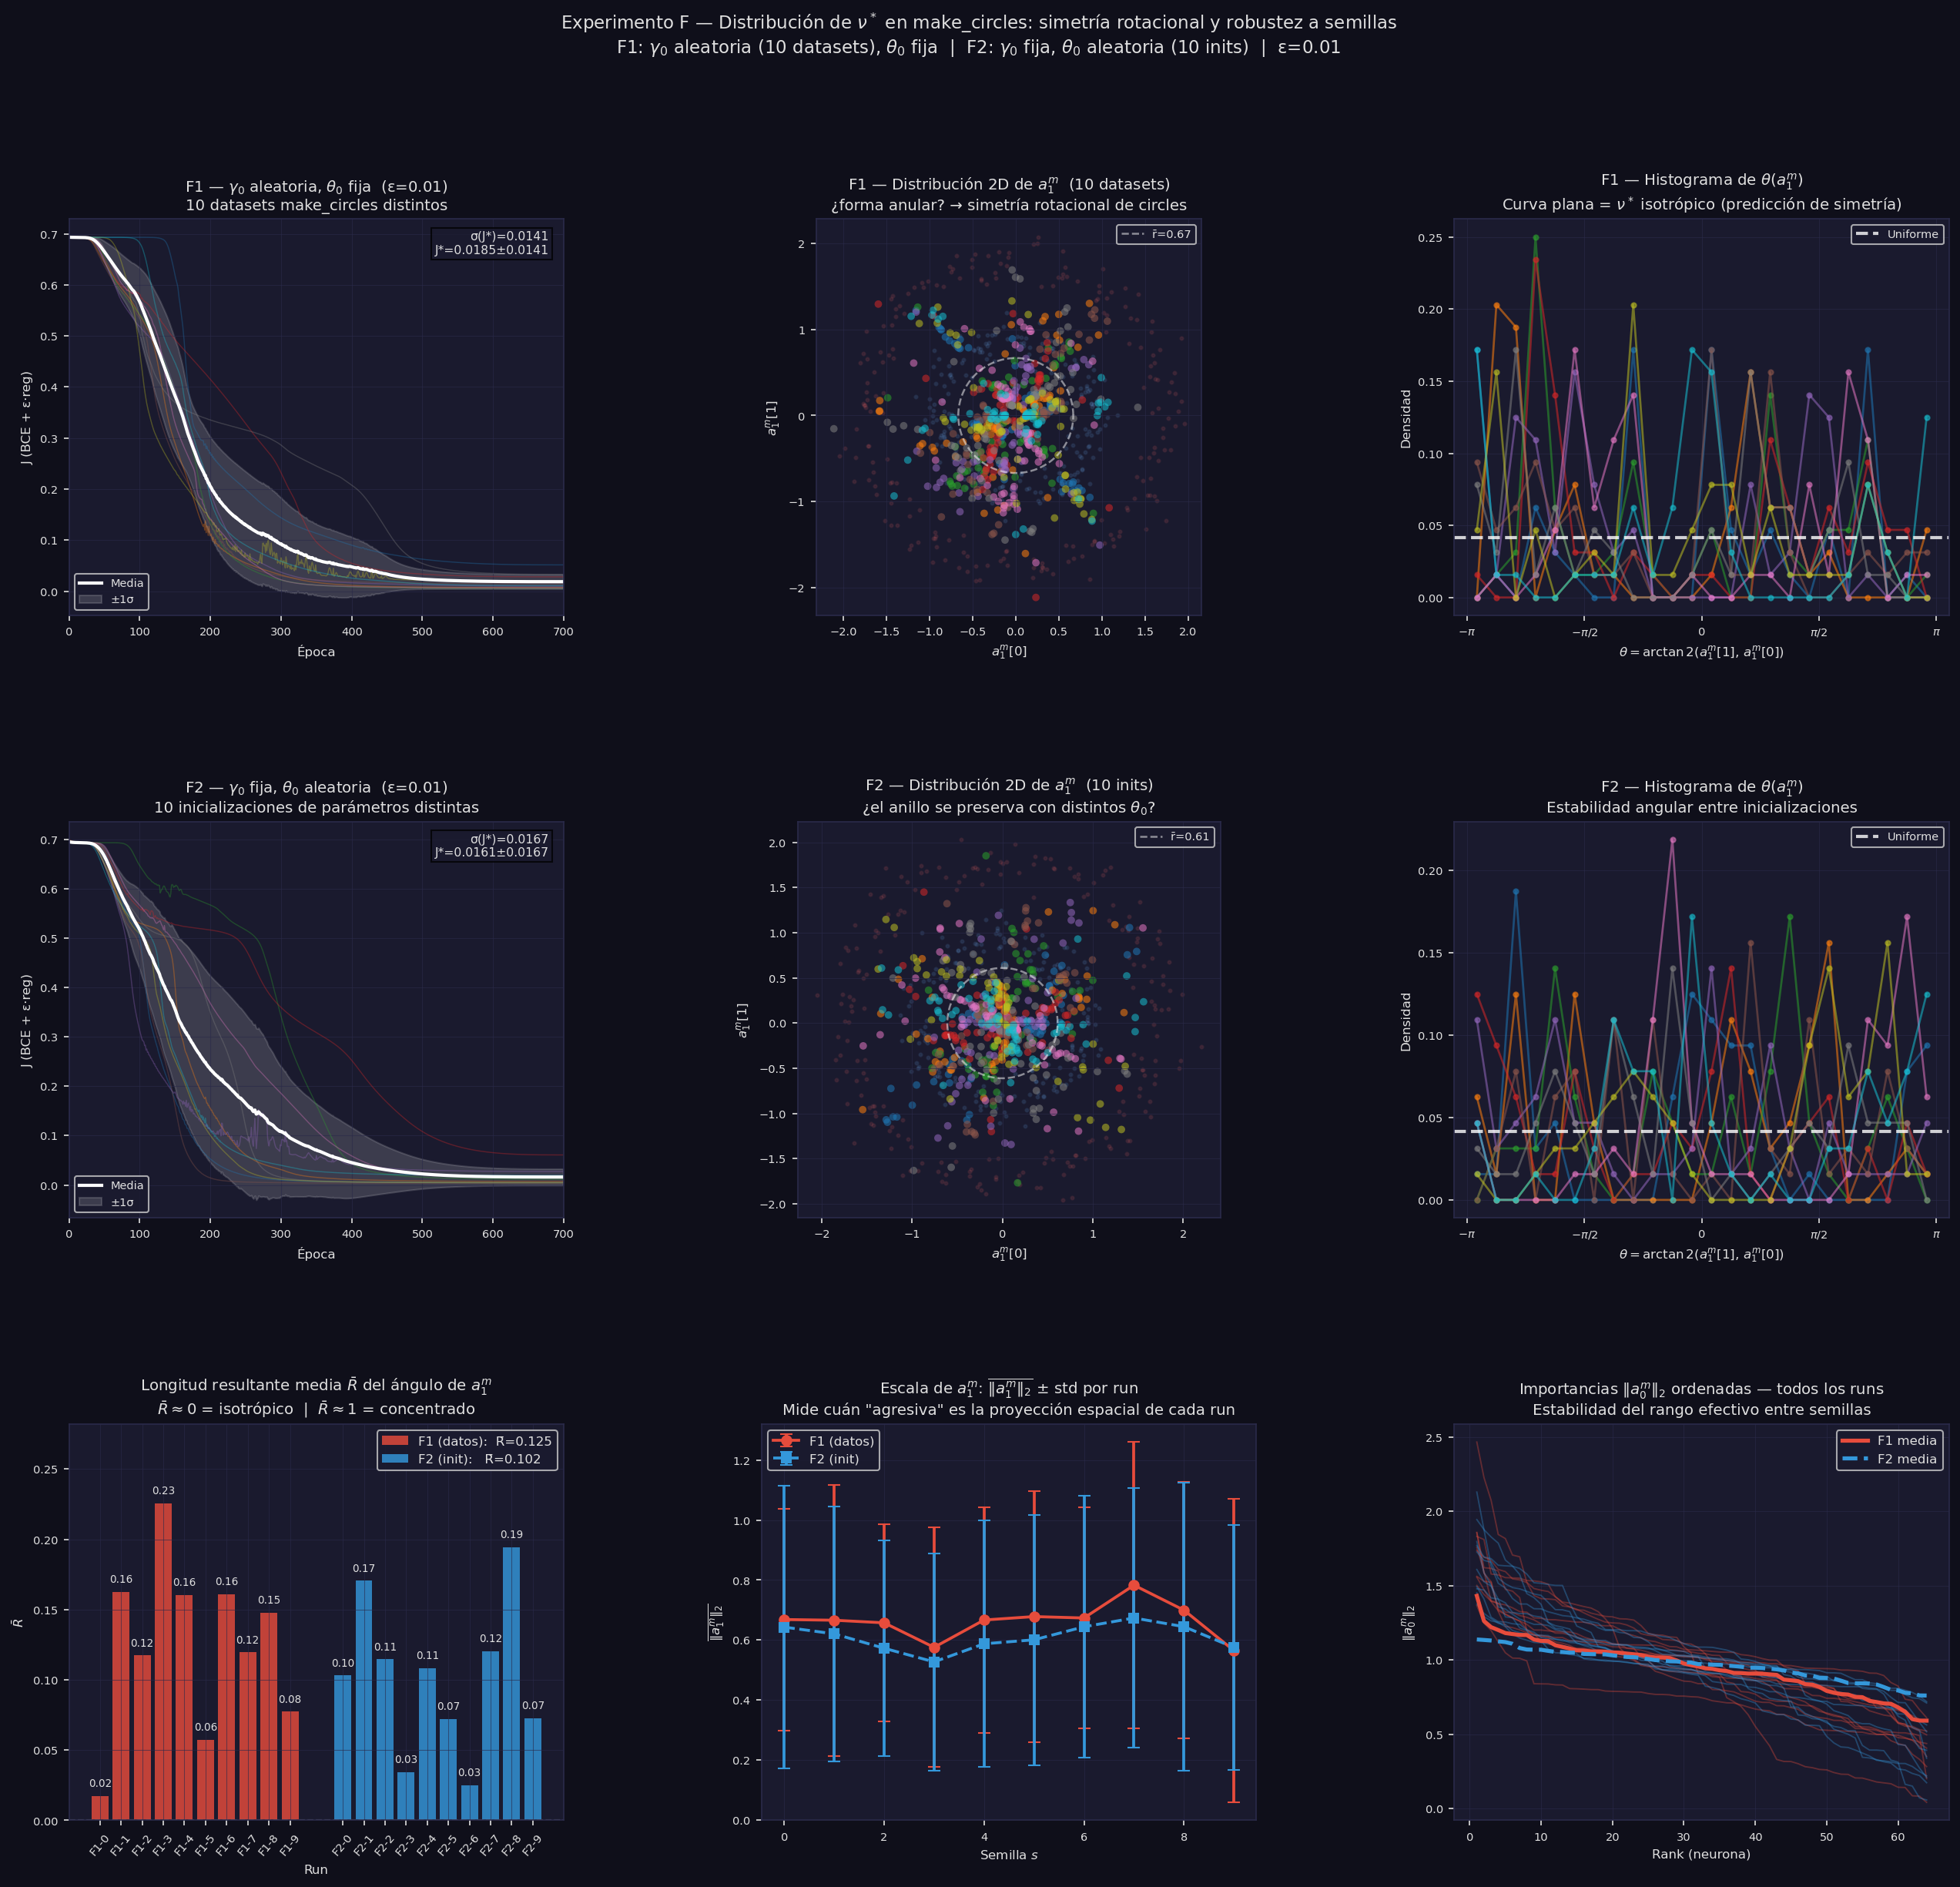
\includegraphics[width=0.95\linewidth]{../figuras/F_circles_parameter_distribution.png}
\end{center}

\end{frame}

% -------------------------------------------------------------------
\begin{frame}{Experimento F — Convergencia y distribución de $a_1^m$}

\begin{columns}
\column{0.55\textwidth}

\textbf{Curvas de convergencia (columna 0):}\\
La mayoría de los runs converge a acc~$\geq 99.5\%$. La banda de F1 (datos variables) es ligeramente más ancha que la de F2 (init variable): en circles, la aleatoriedad del dataset introduce \textbf{más variabilidad} que la inicialización — patrón \textbf{opuesto} al observado en moons con el Experimento D.

\bigskip
\textbf{Scatter 2D de $a_1^m$ (columna 1):}\\
Los vectores $a_1^m$ de los 10 runs (coloreados por run) forman una \textbf{nube difusa} centrada en el origen, sin la estructura bimodal de moons. El círculo discontinuo (radio = norma media) indica que los vectores se sitúan aproximadamente sobre un anillo.

\column{0.41\textwidth}
\begin{block}{Histograma de $\theta$ (columna 2)}
  Distribución del ángulo $\theta^m = \arctan2(a_1^m[1], a_1^m[0])$.

  \medskip
  Las curvas oscilan alrededor de la línea uniforme (blanca discontinua). El ruido es esperado: con $M=64$ y 24 bins hay solo $\sim 2$--$3$ neuronas por bin.

  \medskip
  La \textbf{ausencia de picos sistemáticos} (que sí aparecerían para moons) es la firma de isotropía.
\end{block}
\end{columns}

\end{frame}

% -------------------------------------------------------------------
\begin{frame}{Experimento F — Síntesis: test de isotropía con $\bar{R}$}

\begin{columns}
\column{0.55\textwidth}

\textbf{Panel (2,0) — $\bar{R}$ por run:}

\begin{tabular}{lcc}
  \toprule
  Sub-exp. & $\bar{R}$ (media) & $\bar{R}$ (std) \\
  \midrule
  F1 (datos) & 0.125 & 0.058 \\
  F2 (init)  & 0.102 & 0.051 \\
  \midrule
  Esperado (uniforme) & \multicolumn{2}{c}{$1/\sqrt{64} = 0.125$} \\
  \bottomrule
\end{tabular}

\medskip
Ambos valores son \textbf{consistentes con el nivel de ruido estadístico} de la distribución uniforme en $S^1$. No se puede distinguir $\nu^*$ de la distribución uniforme con $M=64$ neuronas: la predicción de isotropía está verificada hasta el límite de detección.

\column{0.41\textwidth}
\begin{alertblock}{Verificación de la predicción}
  $\bar{R}_{F1} = 0.125 \approx \mathbb{E}[\bar{R}]_{\text{uniforme}}$

  \medskip
  La simetría rotacional de make\_circles \textbf{se transmite a $\nu^*$}: los pesos de entrada $a_1^m$ aprenden a cubrir $S^1$ de forma uniforme, reflejando que ninguna dirección espacial es privilegiada.

  \medskip
  Este resultado es robusto a ambas fuentes de aleatoriedad (F1 y F2).
\end{alertblock}

\medskip
\begin{block}{Importancias: estructura universal}
  Las curvas $\|a_0^m\|_2$ ordenadas son estables entre seeds (F1 y F2). El codo rápido (pocas neuronas dominan) aparece en circles igual que en moons: es una propiedad de la \textbf{arquitectura}, no del dataset.
\end{block}
\end{columns}

\end{frame}

% -------------------------------------------------------------------
\begin{frame}{Experimento F — Comparativa moons vs.\ circles}

\begin{center}
\begin{tabular}{p{0.30\linewidth}p{0.30\linewidth}p{0.30\linewidth}}
  \toprule
  & \textbf{make\_moons} & \textbf{make\_circles} \\
  \midrule
  Simetría de $\gamma_0$ & Reflexión (1 eje) & Rotacional $SO(2)$ \\[6pt]
  Distribución de $a_1^m$ & Bimodal ($\pm 0.3$--$0.4$) & Uniforme en $S^1$ \\[6pt]
  $\bar{R}$ estimado & $> 0.3$ (dos picos) & $0.12$ (ruido de uniforme) \\[6pt]
  Fuente dominante de variabilidad & Inicialización ($\theta_0$) & Dataset ($\gamma_0$) \\[6pt]
  Importancias $\|a_0^m\|$ & Codo rápido & Codo rápido \\
  \bottomrule
\end{tabular}
\end{center}

\bigskip
\begin{block}{Principio general}
  La \textbf{geometría del dataset} determina la estructura de la distribución óptima de parámetros $\nu^*$. El prior $\nu^\infty$ establece el punto de referencia, pero la estructura de $\gamma_0$ «dobla» esa distribución hacia las simetrías del problema. El dataset isotrópico produce $\nu^*$ isotrópico; el dataset bimodal produce $\nu^*$ bimodal.
\end{block}

\end{frame}

% ===================================================================
\section{Conclusiones}

% -------------------------------------------------------------------
\begin{frame}{Conclusiones — Experimentos D, E y F}

\begin{block}{Evidencia empírica: Experimentos D, E, F}
\small
\begin{tabular}{p{0.42\linewidth}p{0.50\linewidth}}
  \toprule
  Resultado / Predicción & Verificación empírica \\
  \midrule
  Genericidad (MT1): minimizador único para casi toda $\gamma_0$ &
    Exp.\ D2/D3: fronteras topológicamente similares en 10 datasets distintos \\[4pt]
  $\varepsilon>0$ hace la unicidad más robusta a $\theta_0$ &
    Exp.\ D1: boxplots de $J^*$ compactos con $\varepsilon=0.01$; dispersos con $\varepsilon=0$ \\[4pt]
  Inicialización domina sobre datos en moons &
    Exp.\ D: std(D1)=0.074~$\gg$~std(D2)=0.026 \\[4pt]
  Tipos de parámetros con distribuciones distintas &
    Exp.\ E fila 0: $a_1^m$ bimodal, $a_0^m$ cola pesada \\[4pt]
  $\varepsilon$ cambia cualitativamente la estructura de $\nu^*$ &
    Exp.\ E: inversión de correlación $r(\|a_1^m\|,\|a_0^m\|)$: $-0.6\to+0.6$ \\[4pt]
  Geometría de $\gamma_0$ determina $\nu^*$ &
    Exp.\ F: circles $\Rightarrow$ $\bar{R}=0.125\approx 1/\sqrt{64}$ (isótropo) \\[4pt]
  Isotropía de $\nu^*$ robusta a semillas &
    Exp.\ F1/F2: $\bar{R}$ estable variando datos e init \\
  \bottomrule
\end{tabular}
\end{block}

\end{frame}

% -------------------------------------------------------------------
\begin{frame}{Conclusiones — El papel de $\varepsilon$ y la simetría}

\begin{columns}
\column{0.48\textwidth}
\begin{block}{El rol de $\varepsilon$ (síntesis D+E)}
  \begin{itemize}
    \item \textbf{Convergencia} (Exp.\ D): $\varepsilon>0$ reduce la dispersión de $J^*$ entre seeds $\Rightarrow$ unicidad más robusta.
    \medskip
    \item \textbf{Estructura de $\nu^*$} (Exp.\ E): $\varepsilon$ invierte la correlación entrada--salida ($r: -0.6 \to +0.6$) y aplanación de la curva de importancias.
    \medskip
    \item $\varepsilon$ no necesita ser grande: \textbf{cualquier $\varepsilon>0$} garantiza la condición PL (Meta-Teorema 2).
  \end{itemize}
\end{block}

\column{0.48\textwidth}
\begin{block}{El rol de la simetría (Exp.\ F)}
  \begin{itemize}
    \item La simetría de $\gamma_0$ se «imprime» en $\nu^*$ a través del entrenamiento.
    \medskip
    \item make\_moons (reflexión) $\to$ $a_1^m$ bimodal.
    \medskip
    \item make\_circles ($SO(2)$) $\to$ $a_1^m$ uniforme en $S^1$.
    \medskip
    \item La estructura de importancias ($\|a_0^m\|_2$) es \textbf{universal}: depende de la arquitectura, no del dataset.
  \end{itemize}
\end{block}
\end{columns}

\bigskip
\begin{alertblock}{Mensaje central}
  La teoría de Daudin \& Delarue (2025) no solo predice convergencia: también estructura la distribución de parámetros aprendida. Los experimentos D, E y F son verificaciones cuantitativas de esas predicciones.
\end{alertblock}

\end{frame}

% -------------------------------------------------------------------
\begin{frame}{Referencias}

\begin{thebibliography}{9}
\bibitem{daudin2025}
  Daudin, S.\ \& Delarue, F.\ (2025).
  \textit{Genericity of the Polyak-Łojasiewicz inequality for mean-field Neural ODEs with entropic regularization.}
  arXiv:2507.08486.

\bibitem{chen2018}
  Chen, R.T.Q., Rubanova, Y., Bettencourt, J.\ \& Duvenaud, D.\ (2018).
  \textit{Neural Ordinary Differential Equations.}
  NeurIPS 2018.

\bibitem{polyak1963}
  Polyak, B.T.\ (1963).
  \textit{Gradient methods for the minimisation of functionals.}
  USSR Computational Mathematics and Mathematical Physics, 3(4), 864--878.

\bibitem{mardia2000}
  Mardia, K.V.\ \& Jupp, P.E.\ (2000).
  \textit{Directional Statistics.}
  Wiley.
  (\textit{Estadística circular: definición de $\bar{R}$ y test de Rayleigh.})
\end{thebibliography}

\end{frame}

% -------------------------------------------------------------------
\begin{frame}{}
  \begin{center}
    \Large\textbf{Gracias}\\[1em]
    \normalsize
    Código disponible en:\\
    \texttt{daudin\_delarue\_moons.py}\\[1em]
    Beca JAE Intro — CSIC\\
    Tutor: Rafael Orive
  \end{center}
\end{frame}

\end{document}
